\documentclass[11pt, oneside, a4paper]{article}

%--- PREAMBLE ---%
\usepackage{geometry}
\usepackage[utf8]{inputenc}
\usepackage[T1]{fontenc}
\usepackage{hyperref}
\usepackage{float}
\usepackage{amsmath}
\usepackage{pgfplots}
\pgfplotsset{width=10cm,compat=1.9}

\setcounter{tocdepth}{2}
\hypersetup{
	hidelinks
}

\title{CMPE 300: Project 1}
\author{
	Buğra Keser\\2021400144
	\and
	Yusuf Anıl Yazıcı\\2021400207
}
\date{\today}

%-- DOCUMENT ---%

\begin{document}
	\maketitle

	\tableofcontents

	\newpage

	\section{Theoretical Analysis}


\subsection{Basic operation is the comparison marked as (1)}
Assuming that the comparison marked as (1) is the basic operation, the number of basic operations remains the same for all cases, as the comparison is executed with every increment in the for loop, regardless of any other operations and input types.

\subsubsection{Analysis of B(n)}
As the for loop executes \( n \) times, the comparison is also executed \( n \) times. Therefore, the number of basic operations is \( n \), which implies asymptotic notation of \(\boldsymbol{\theta(n)}\).

\subsubsection{Analysis of W(n)}
As the for loop executes \( n \) times, the comparison is also executed \( n \) times. Therefore, the number of basic operations is \( n \), which implies asymptotic notation of \(\boldsymbol{\theta(n)}\).

\subsubsection{Analysis of A(n)}
As the for loop executes \( n \) times, the comparison is also executed \( n \) times. Therefore, the number of basic operations is \( n \), which implies asymptotic notation of \(\boldsymbol{\theta(n)}\).


	\subsection{Basic operations are the two loop increments marked as (2)}

	\subsubsection{Analysis of B(n)}
The best case for the input occurs when all elements of the array are either 'm' or 'p', as the marked basic operations are never executed. This is because the corresponding \texttt{if} conditions that trigger the execution of the marked operations are never satisfied. Thus, the number of basic operations for such an input is 0, which implies asymptotic notation of \(\boldsymbol{\theta(1)}\).

	\subsubsection{Analysis of W(n)}
 
The worst-case scenario occurs when the array consists only of 'c' letters, as this triggers the execution of the basic operation based on the input size each time, unlike the 'e' case, which depends on the index of the letter. This ensures that the basic operation is executed more frequently. 

The y-value of the inner for loop jumps \( j \) times—which depends on the value of \( i \) in the outer loop—every time it is iterated, yielding the following equation: \(( n +  \sum_{i=1}^{n} \lfloor\frac{n}{i} \rfloor)\).


\begin{flushleft}
Taking into account the outer loop, which executes n times, the notation for the analysis is as follows:
\[
n \cdot \left( n +  \sum_{i=1}^{n} \lfloor \frac{n}{i} \rfloor \right)
\]
\end{flushleft}
The summation notation \(\sum_{i=1}^{n} \lfloor \frac{n}{i} \rfloor\) yields \(\theta(n \log n)\) due to the harmonic series' behavior when summed over all \( i \). Since this term is multiplied by \( n \) in the final expression \( n \cdot \left( n + \sum_{i=1}^{n} \lfloor \frac{n}{i} \rfloor \right) \), the resulting time complexity becomes \(\theta(n^2 \log n)\). This is because multiplying \(\theta(n \log n)\) by \( n \) scales the complexity to \(\boldsymbol{\theta(n^2 \log n)}\).


	\subsubsection{Analysis of A(n)}
 The average case analysis requires considering the probability distribution of the different input elements ('c', 'm', 'p', 'e') and the number of times the basic operations are executed for each scenario. The notation for the analysis is given by:

\begin{equation*}
\frac{n}{8} \cdot \left( n + n \sum_{i=1}^{n} \frac{1}{i} \right) + \frac{n}{4} \cdot 0 + \frac{n}{8} \cdot 0 + \frac{1}{2} \sum_{i=0}^{n-1} i
\end{equation*}

Breaking down this equation:

1. **Contribution of 'c' (with probability \(\frac{1}{8}\))**:
   \[
   \frac{n}{8} \cdot \left( n + n \sum_{i=1}^{n} \frac{1}{i} \right)
   \]
   This term contributes \(\theta(n^2 \log n)\) as the summation \(\sum_{i=1}^{n} \frac{1}{i}\) yields \(\theta(\log n)\) when summed, and multiplying by \( n \) scales it to \(\theta(n \log n)\). Multiplying by \( \frac{n}{8} \) results in \(\theta(n^2 \log n)\).

2. **Contribution of 'm' and 'p' (with probabilities \(\frac{1}{4}\) and \(\frac{1}{8}\))**:
   \[
   \frac{n}{4} \cdot 0 + \frac{n}{8} \cdot 0
   \]
   These terms do not contribute to the basic operations as they yield 0.

3. **Contribution of 'e' (with probability \(\frac{1}{2}\))**:
   \[
   \frac{1}{2} \sum_{i=0}^{n-1} i
   \]
   This term simplifies to \(\frac{1}{2} \cdot \frac{(n-1)n}{2}\), which is \(\theta(n^2)\).

Combining these contributions:

\[
\theta\left(\frac{n}{8} \cdot (n + n \log n)\right) + \theta\left(\frac{1}{2} \cdot \frac{(n-1)n}{2}\right)
\]

The dominant term here is \(\theta(n^2 \log n)\), as it grows faster than \(\theta(n^2)\). Therefore, the final average case complexity is:

\[
\boldsymbol{\theta(n^2 \log n)}
\]
\noindent The notation for the analysis is as follows:
\begin{equation*}
\frac{n}{8} \cdot \left( n + n \sum_{i=1}^{n} \frac{1}{i} \right) + \frac{n}{4} \cdot 0 + \frac{n}{8} \cdot 0 + \frac{1}{2} \sum_{i=0}^{n-1} i
\end{equation*}

	\subsection{Basic operations are the four assignments marked as (3)}

	\subsubsection{Analysis of B(n)}
\noindent The notation for the analysis is as follows:
\begin{equation*}
0 + (n-1) \cdot \left( \lfloor \log_5 n \rfloor + 1 \right)
\end{equation*}
	\subsubsection{Analysis of W(n)}
 \noindent The expression is as follows:
\begin{equation*}
\frac{n^3 - n}{3} + n
\end{equation*}

        \subsubsection{Analysis of A(n)}
        \noindent The expression is as follows:
\begin{equation*}
\frac{n}{8} \cdot n + \frac{n}{4} \cdot \lceil \log_2 n \rceil + \frac{n}{8} \cdot \left( \lfloor \log_5 n \rfloor + 1 \right) + \frac{n^3 - n}{6}
\end{equation*}


	\subsection{Basic operations are the four assignments marked as (4)}

	\subsubsection{Analysis of B(n)}
 \noindent The notation for the analysis is as follows:
\begin{equation*}
0 + (n-1) \cdot \left( \lfloor \log_5 n \rfloor + 1 \right)
\end{equation*}

	\subsubsection{Analysis of W(n)}
 \noindent The expression is as follows:
\begin{equation*}
\left( n + n \sum_{i=1}^{n} \frac{1}{i} \right) + \frac{n^4 - n^2}{3}
\end{equation*}

	
        \subsubsection{Analysis of A(n)}
        \begin{equation*}
\frac{n}{8} \cdot ( n + n \sum_{i=1}^{n} \frac{1}{i} ) + \frac{n}{4} \cdot \lceil \log_2 n \rceil + \frac{n}{8} \cdot \left( \lfloor \log_5 n \rfloor + 1 \right) + \frac{n^4 - n^2}{6}
\end{equation*}

	\section{Identification of Basic Operation(s)}

The assignments marked as (4) were chosen as the basic operations because they are executed within nested loops that contribute significantly to the overall computational effort of the algorithm. These assignments directly impact the total runtime as they are repeated multiple times based on the input size \( n \) and the structure of the algorithm. 

	\section{Real Execution}

	\begin{table}[H]
		\centering
		\begin{tabular}{|l|l|} \hline
			\textbf{N Size} & \textbf{Time Elapsed (sec)} \\ \hline
			1 & \( 7.15 \times 10^{-7}\) \\ \hline
			5 & \( 1.00 \times 10^{-6}\) \\ \hline
			10 & \( 1.07 \times 10^{-6}\) \\ \hline
			20 & \( 1.98 \times 10^{-6}\) \\ \hline
			30 & \( 3.96 \times 10^{-6}\) \\ \hline
			40 & \( 4.94 \times 10^{-6}\) \\ \hline
			50 & \( 6.03 \times 10^{-6}\) \\ \hline
			60 & \( 7.30 \times 10^{-6}\) \\ \hline
			70 & \( 9.11 \times 10^{-6}\) \\ \hline
			90 & \( 1.08 \times 10^{-5}\) \\ \hline
			100 & \( 1.22 \times 10^{-5}\) \\ \hline
			120 & \( 1.45 \times 10^{-5}\) \\ \hline
			130 & \( 2.30 \times 10^{-5}\) \\ \hline
			140 & \( 2.39 \times 10^{-5}\) \\ \hline
			150 & \( 2.66 \times 10^{-5}\) \\ \hline
			160 & \( 2.80 \times 10^{-5}\) \\ \hline
			170 & \( 3.20 \times 10^{-5}\) \\ \hline
		\end{tabular}
		\caption{Best Case Real Execution Times}
		\label{tab:best-case}
	\end{table}


	\begin{table}[H]
		\centering
		\begin{tabular}{|l|l|} \hline
			\textbf{N Size} & \textbf{Time Elapsed (sec)} \\ \hline
			1 & \( 5.72 \times 10^{-7}\) \\ \hline
			5 & \( 7.72 \times 10^{-6}\) \\ \hline
			10 & \( 8.43 \times 10^{-5}\) \\ \hline
			20 & \( 1.33 \times 10^{-3}\) \\ \hline
			30 & \( 6.52 \times 10^{-3}\) \\ \hline
			40 & \( 2.01 \times 10^{-2}\) \\ \hline
			50 & \( 4.80 \times 10^{-2}\) \\ \hline
			60 & \( 9.83 \times 10^{-2}\) \\ \hline
			70 & \( 1.85 \times 10^{-1}\) \\ \hline
			90 & \( 5.01 \times 10^{-1}\) \\ \hline
			100 & \( 7.55 \times 10^{-1}\) \\ \hline
			120 & \( 1.54 \) \\ \hline
			130 & \( 2.11 \) \\ \hline
			140 & \( 2.84 \) \\ \hline
			150 & \( 3.74 \) \\ \hline
			160 & \( 4.82 \) \\ \hline
			170 & \( 6.12 \) \\ \hline
		\end{tabular}
		\caption{Worst Case Real Execution Times}
		\label{tab:worst-case}
	\end{table}

	\begin{table}[H]
		\centering
		\begin{tabular}{|l|l|} \hline
			\textbf{N Size} & \textbf{Time Elapsed (sec)} \\ \hline
			1 & \( 5.96 \times 10^{-7}\) \\ \hline
			5 & \( 5.53 \times 10^{-6}\) \\ \hline
			10 & \( 5.39 \times 10^{-5}\) \\ \hline
			20 & \( 7.34 \times 10^{-4}\) \\ \hline
			30 & \( 3.45 \times 10^{-3}\) \\ \hline
			40 & \( 9.99 \times 10^{-3}\) \\ \hline
			50 & \( 2.88 \times 10^{-2}\) \\ \hline
			60 & \( 5.49 \times 10^{-2}\) \\ \hline
			70 & \( 1.32 \times 10^{-1}\) \\ \hline
			90 & \( 2.54 \times 10^{-1}\) \\ \hline
			100 & \( 4.06 \times 10^{-1}\) \\ \hline
			120 & \( 8.01 \times 10^{-1}\) \\ \hline
			130 & \( 1.13 \) \\ \hline
			140 & \( 1.46 \) \\ \hline
			150 & \( 2.01 \) \\ \hline
			160 & \( 2.53 \) \\ \hline
			170 & \( 3.26 \) \\ \hline
		\end{tabular}
		\caption{Average Case Real Execution Times}
		\label{tab:avg-case}
	\end{table}

	\section{Comparison}

	\subsection{Best Case}

	\subsubsection{Graph of the real execution time of the algorithm}

	% Here is an example line plot of data points for you. Feel free to change it or use something else.

	\begin{figure}[H]
	\centering
	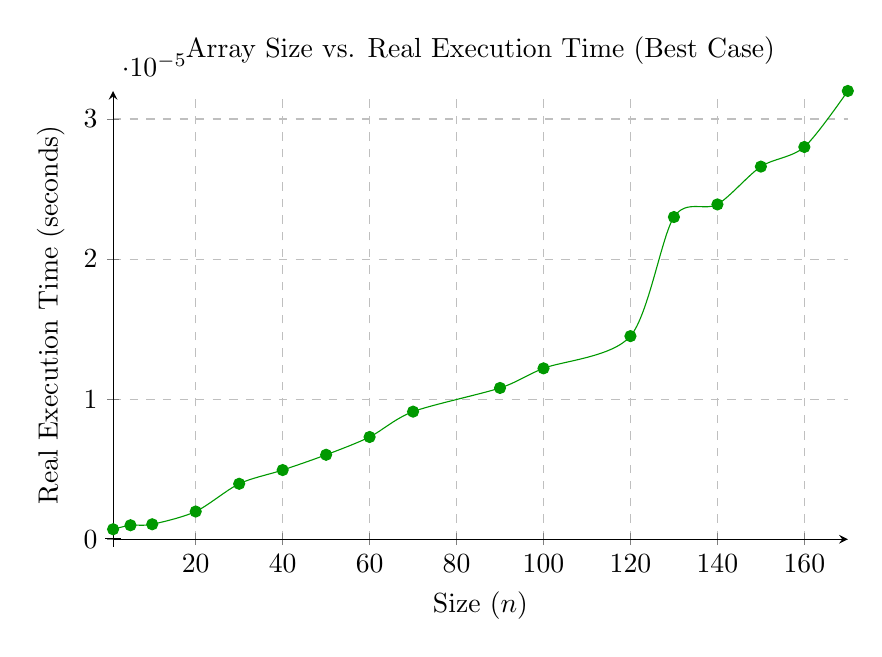
\begin{tikzpicture}
		\begin{axis}[
			% Axis labels and title
			title={Array Size vs. Real Execution Time (Best Case)},
			xlabel={Size (\(n\))},
			ylabel={Real Execution Time (seconds)},
			% Axis limits
			%xmin=0, xmax=100,
			ymin=0, %ymax=200,
			% Axis ticks
			% xtick={0,20,40,60,80,100},
			% ytick={0,20,40,60,80,100,120},
			grid=both,
			axis lines=left,
			axis line style={|-stealth},
			grid style=dashed,
			width=0.9\textwidth,
			height=\axisdefaultheight
			]
			\addplot[
				color=green!60!black,
				mark=*,
				smooth
				]
			% Change the coordinates here with your own data:
			coordinates {
				(1, 0.000000715)
				(5,   0.00000100)
				(10,  0.00000107)
				(20,  0.00000198)
				(30,  0.00000396)
				(40,  0.00000494)
				(50,  0.00000603)
				(60,  0.00000730)
				(70,  0.00000911)
				(90,  0.0000108)
				(100, 0.0000122)
				(120, 0.0000145)
				(130, 0.0000230)
				(140, 0.0000239)
				(150, 0.0000266)
				(160, 0.0000280)
				(170, 0.0000320)
			};
		\end{axis}
	\end{tikzpicture}
	\end{figure}

	\subsubsection{Graph of the theoretical analysis when basic operation is the operation marked as (1)}

    \begin{figure}[H]
	\centering
	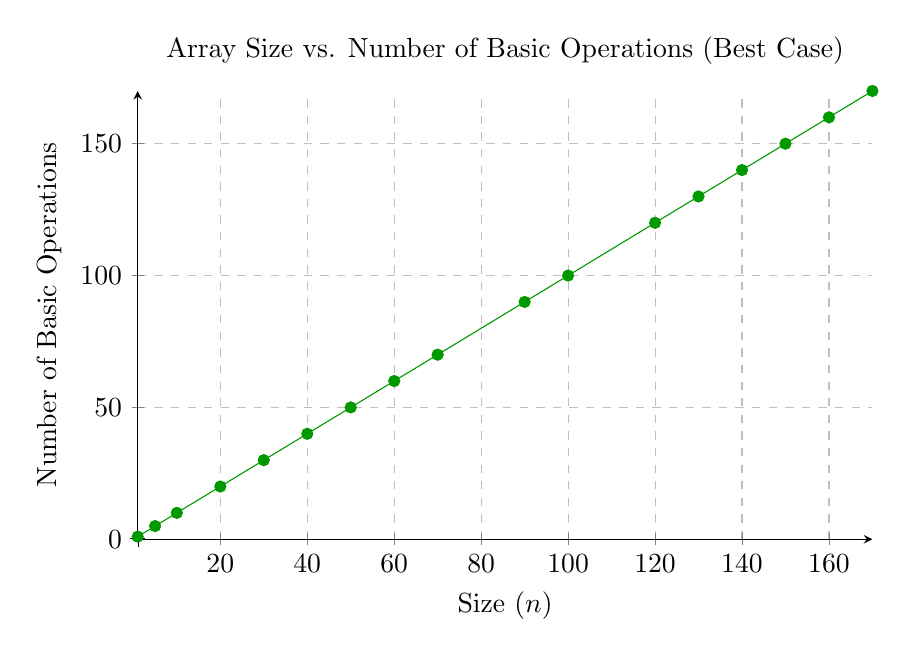
\begin{tikzpicture}
		\begin{axis}[
			% Axis labels and title
			title={Array Size vs. Number of Basic Operations (Best Case)},
			xlabel={Size (\(n\))},
			ylabel={Number of Basic Operations},
			% Axis limits
			%xmin=0, xmax=100,
			ymin=0, %ymax=200,
			% Axis ticks
			% xtick={0,20,40,60,80,100},
			% ytick={0,20,40,60,80,100,120},
			grid=both,
			axis lines=left,
			axis line style={|-stealth},
			grid style=dashed,
			width=0.9\textwidth,
			height=\axisdefaultheight
			]
			\addplot[
				color=green!60!black,
				mark=*,
				smooth
				]
			% Change the coordinates here with your own data:
			coordinates {
				(1,   1)
				(5,   5)
				(10,  10)
				(20, 20)
				(30,  30)
				(40, 40)
				(50,  50)
				(60,  60)
				(70,  70)
				(90,  90)
				(100,100)
				(120, 120)
				(130, 130)
				(140, 140)
				(150, 150)
				(160, 160)
				(170,170)
			};
		\end{axis}
	\end{tikzpicture}
	\end{figure}

	\subsubsection{Graph of the theoretical analysis when basic operation is the operation marked as (2)}

 \begin{figure}[H]
	\centering
	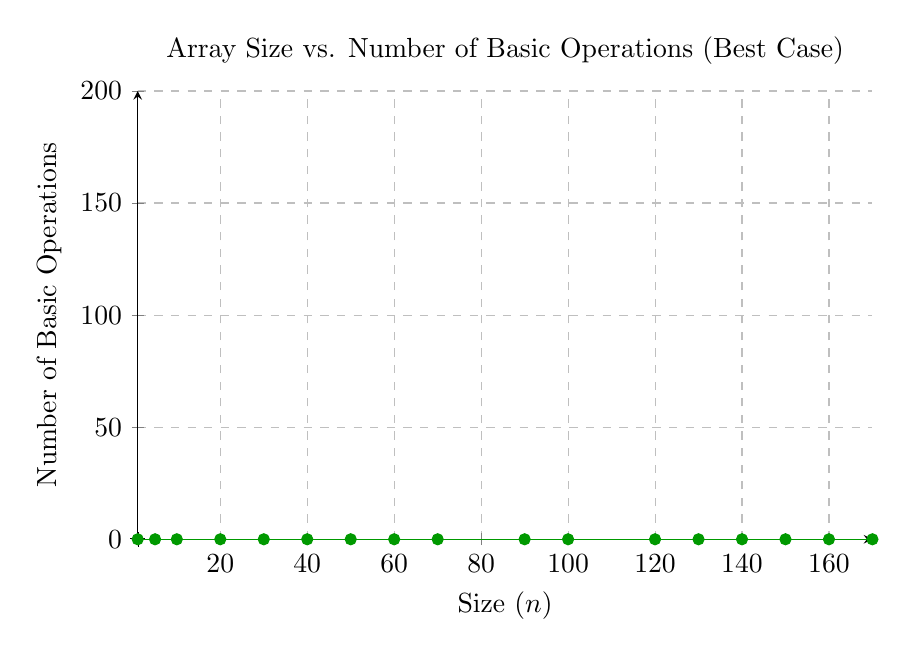
\begin{tikzpicture}
		\begin{axis}[
			% Axis labels and title
			title={Array Size vs. Number of Basic Operations (Best Case)},
			xlabel={Size (\(n\))},
			ylabel={Number of Basic Operations},
			%Axis limits
			%xmin=0, xmax=100,
		    ymin=0, ymax=200,
			% Axis ticks
			% xtick={0,20,40,60,80,100},
			% ytick={0,20,40,60,80,100,120},
			grid=both,
			axis lines=left,
			axis line style={|-stealth},
			grid style=dashed,
			width=0.9\textwidth,
			height=\axisdefaultheight
			]
			\addplot[
				color=green!60!black,
				mark=*,
				smooth
				]
			% Change the coordinates here with your own data:
			coordinates {
				(1,   0)
				(5,   0)
				(10,  0)
				(20, 0)
				(30,  0)
				(40, 0)
				(50,  0)
				(60,  0)
				(70,  0)
				(90,  0)
				(100,0)
				(120, 0)
				(130, 0)
				(140, 0)
				(150, 0)
				(160, 0)
				(170,0)
			};
		\end{axis}
	\end{tikzpicture}
	\end{figure}

	\subsubsection{Graph of the theoretical analysis when basic operation is the operation marked as (3)}

 \begin{figure}[H]
	\centering
	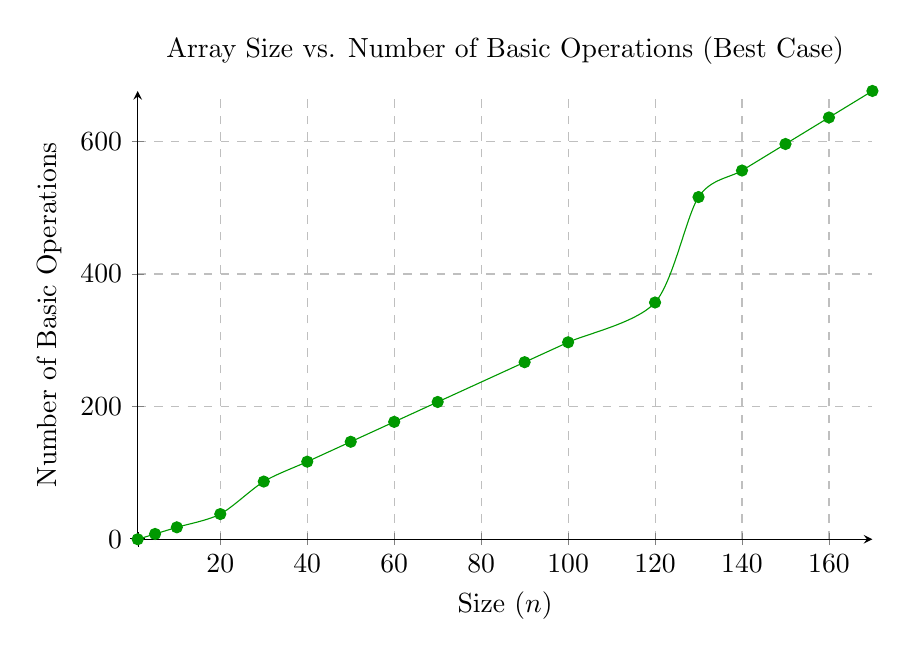
\begin{tikzpicture}
		\begin{axis}[
			% Axis labels and title
			title={Array Size vs. Number of Basic Operations (Best Case)},
			xlabel={Size (\(n\))},
			ylabel={Number of Basic Operations},
			% Axis limits
			%xmin=0, xmax=100,
			ymin=0, %ymax=200,
			% Axis ticks
			% xtick={0,20,40,60,80,100},
			% ytick={0,20,40,60,80,100,120},
			grid=both,
			axis lines=left,
			axis line style={|-stealth},
			grid style=dashed,
			width=0.9\textwidth,
			height=\axisdefaultheight
			]
			\addplot[
				color=green!60!black,
				mark=*,
				smooth
				]
			% Change the coordinates here with your own data:
			coordinates {
				(1, 0  )
				(5,  8 )
				(10, 18  )
				(20, 38)
				(30, 87 )
				(40,117 )
				(50, 147 )
				(60, 177 )
				(70, 207 )
				(90, 267 )
				(100,297)
				(120,357)
				(130, 516)
				(140,556 )
				(150, 596)
				(160,636 )
				(170,676)
			};
		\end{axis}
	\end{tikzpicture}
	\end{figure}

	\subsubsection{Graph of the theoretical analysis when basic operation is the operation marked as (4)}

 \begin{figure}[H]
	\centering
	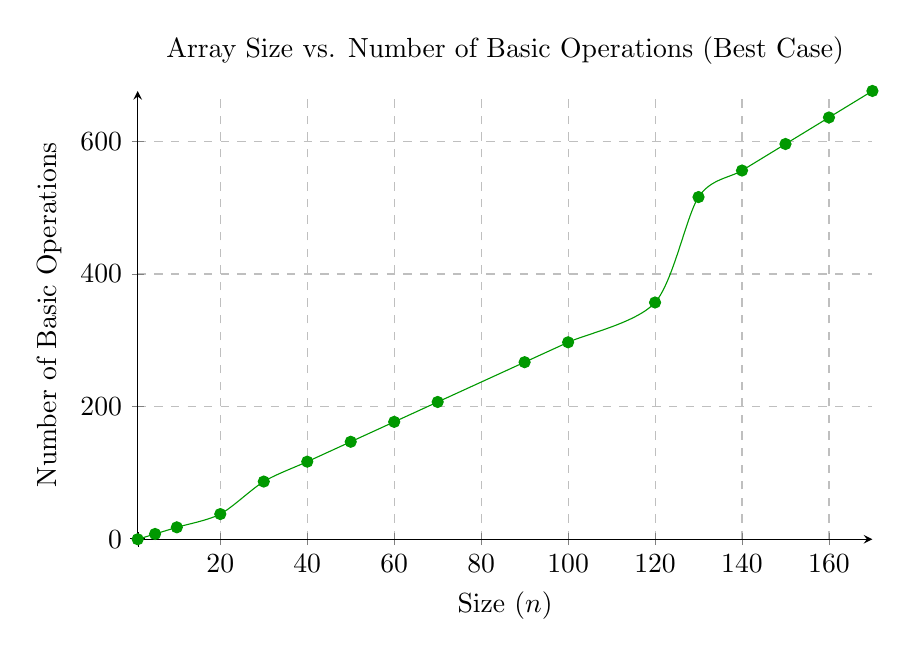
\begin{tikzpicture}
		\begin{axis}[
			% Axis labels and title
			title={Array Size vs. Number of Basic Operations (Best Case)},
			xlabel={Size (\(n\))},
			ylabel={Number of Basic Operations},
			% Axis limits
			%xmin=0, xmax=100,
			ymin=0, %ymax=200,
			% Axis ticks
			% xtick={0,20,40,60,80,100},
			% ytick={0,20,40,60,80,100,120},
			grid=both,
			axis lines=left,
			axis line style={|-stealth},
			grid style=dashed,
			width=0.9\textwidth,
			height=\axisdefaultheight
			]
			\addplot[
				color=green!60!black,
				mark=*,
				smooth
				]
			% Change the coordinates here with your own data:
			coordinates {
				(1, 0  )
				(5,  8 )
				(10, 18  )
				(20, 38)
				(30, 87 )
				(40,117 )
				(50, 147 )
				(60, 177 )
				(70, 207 )
				(90, 267 )
				(100,297)
				(120,357)
				(130, 516)
				(140,556 )
				(150, 596)
				(160,636 )
				(170,676)
			};
		\end{axis}
	\end{tikzpicture}
	\end{figure}


	\subsubsection{Comments}



	\subsection{Worst Case}

	\subsubsection{Graph of the real execution time of the algorithm}

 \begin{figure}[H]
	\centering
	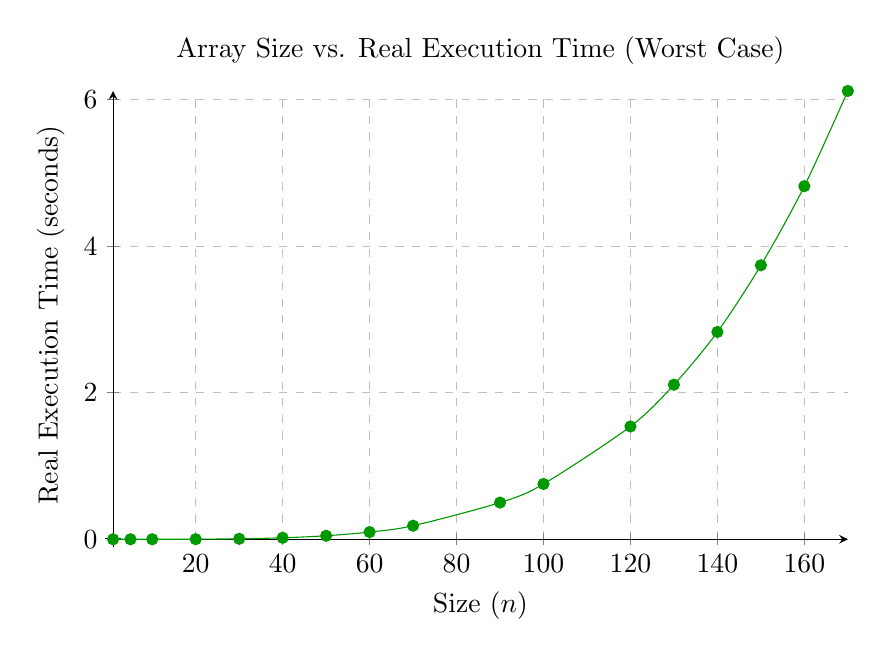
\begin{tikzpicture}
		\begin{axis}[
			% Axis labels and title
			title={Array Size vs. Real Execution Time (Worst Case)},
			xlabel={Size (\(n\))},
			ylabel={Real Execution Time (seconds)},
			% Axis limits
			%xmin=0, xmax=100,
			ymin=0, %ymax=200,
			% Axis ticks
			% xtick={0,20,40,60,80,100},
			% ytick={0,20,40,60,80,100,120},
			grid=both,
			axis lines=left,
			axis line style={|-stealth},
			grid style=dashed,
			width=0.9\textwidth,
			height=\axisdefaultheight
			]
			\addplot[
				color=green!60!black,
				mark=*,
				smooth
				]
			% Change the coordinates here with your own data:
			coordinates {
				(1,   0.000000572)
				(5,   0.00000772)
				(10,  0.0000843)
				(20,  0.00133)
				(30,  0.00652)
				(40,  0.0201)
				(50,  0.0480)
				(60,  0.0983)
				(70,  0.185)
				(90,  0.501)
				(100, 0.755)
				(120, 1.54)
				(130, 2.11)
				(140, 2.83)
				(150, 3.74)
				(160, 4.82)
				(170, 6.12)
			};
		\end{axis}
	\end{tikzpicture}
	\end{figure}

	\subsubsection{Graph of the theoretical analysis when basic operation is the operation marked as (1)}

  \begin{figure}[H]
	\centering
	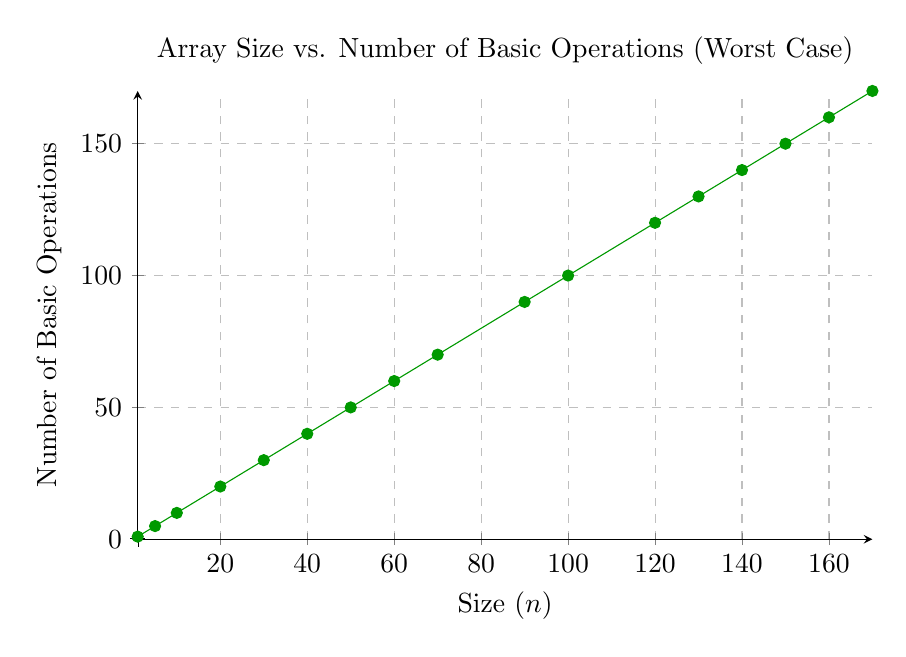
\begin{tikzpicture}
		\begin{axis}[
			% Axis labels and title
			title={Array Size vs. Number of Basic Operations (Worst Case)},
			xlabel={Size (\(n\))},
			ylabel={Number of Basic Operations},
			% Axis limits
			%xmin=0, xmax=100,
			ymin=0, %ymax=200,
			% Axis ticks
			% xtick={0,20,40,60,80,100},
			% ytick={0,20,40,60,80,100,120},
			grid=both,
			axis lines=left,
			axis line style={|-stealth},
			grid style=dashed,
			width=0.9\textwidth,
			height=\axisdefaultheight
			]
			\addplot[
				color=green!60!black,
				mark=*,
				smooth
				]
			% Change the coordinates here with your own data:
			coordinates {
				(1,   1)
				(5,   5)
				(10,  10)
				(20, 20)
				(30,  30)
				(40, 40)
				(50,  50)
				(60,  60)
				(70,  70)
				(90,  90)
				(100,100)
				(120, 120)
				(130, 130)
				(140, 140)
				(150, 150)
				(160, 160)
				(170,170)
			};
		\end{axis}
	\end{tikzpicture}
	\end{figure}

	\subsubsection{Graph of the theoretical analysis when basic operation is the operation marked as (2)}

 \begin{figure}[H]
	\centering
	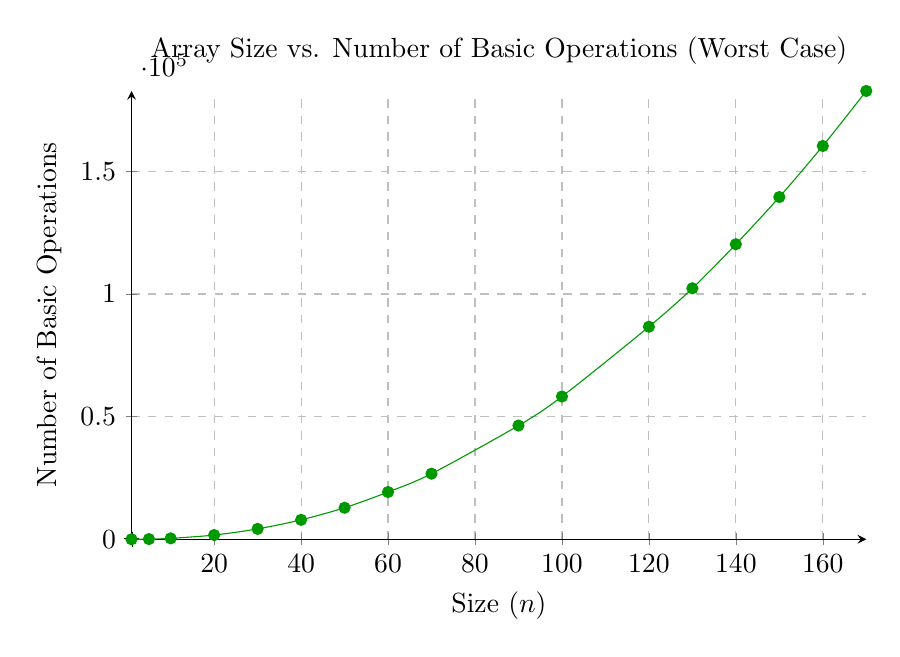
\begin{tikzpicture}
		\begin{axis}[
			% Axis labels and title
			title={Array Size vs. Number of Basic Operations (Worst Case)},
			xlabel={Size (\(n\))},
			ylabel={Number of Basic Operations},
			% Axis limits
			%xmin=0, xmax=100,
			ymin=0, %ymax=200,
			% Axis ticks
			% xtick={0,20,40,60,80,100},
			% ytick={0,20,40,60,80,100,120},
			grid=both,
			axis lines=left,
			axis line style={|-stealth},
			grid style=dashed,
			width=0.9\textwidth,
			height=\axisdefaultheight
			]
			\addplot[
				color=green!60!black,
				mark=*,
				smooth
				]
			% Change the coordinates here with your own data:
			coordinates {
				(1,   2)
				(5,   75)
				(10,  370)
				(20, 1720)
				(30,  4230)
				(40, 7920)
				(50,  12850)
				(60,  19260)
				(70,  26740)
				(90,  46350)
				(100,58200)
				(120, 86640)
				(130, 102310)
				(140, 120260)
				(150, 139500)
				(160, 160320)
				(170,182750)
			};
		\end{axis}
	\end{tikzpicture}
	\end{figure}

	\subsubsection{Graph of the theoretical analysis when basic operation is the operation marked as (3)}

 \begin{figure}[H]
	\centering
	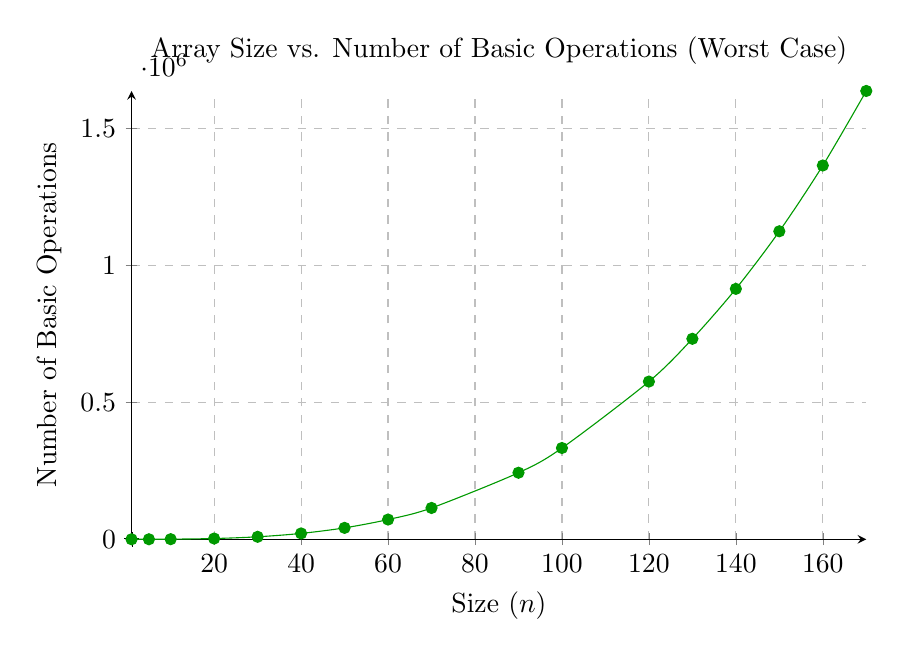
\begin{tikzpicture}
		\begin{axis}[
			% Axis labels and title
			title={Array Size vs. Number of Basic Operations (Worst Case)},
			xlabel={Size (\(n\))},
			ylabel={Number of Basic Operations},
			% Axis limits
			%xmin=0, xmax=100,
			ymin=0, %ymax=200,
			% Axis ticks
			% xtick={0,20,40,60,80,100},
			% ytick={0,20,40,60,80,100,120},
			grid=both,
			axis lines=left,
			axis line style={|-stealth},
			grid style=dashed,
			width=0.9\textwidth,
			height=\axisdefaultheight
			]
			\addplot[
				color=green!60!black,
				mark=*,
				smooth
				]
			% Change the coordinates here with your own data:
			coordinates {
				(1,   1)
				(5,   45)
				(10,  340)
				(20, 2680)
				(30,  9020)
				(40, 21360)
				(50,  41700)
				(60,  72040)
				(70,  114380)
				(90,  243060)
				(100,333400)
				(120, 576080)
				(130, 732420)
				(140, 914760)
				(150, 1125100)
				(160, 1365440)
				(170,1637780)
			};
		\end{axis}
	\end{tikzpicture}
	\end{figure}

	\subsubsection{Graph of the theoretical analysis when basic operation is the operation marked as (4)}

  \begin{figure}[H]
	\centering
	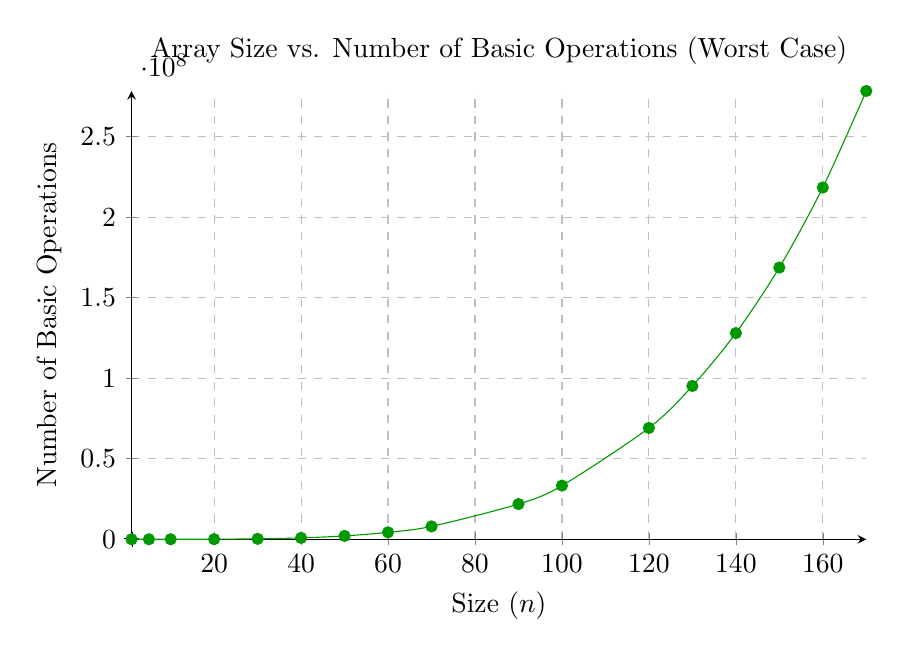
\begin{tikzpicture}
		\begin{axis}[
			% Axis labels and title
			title={Array Size vs. Number of Basic Operations (Worst Case)},
			xlabel={Size (\(n\))},
			ylabel={Number of Basic Operations},
			% Axis limits
			%xmin=0, xmax=100,
			ymin=0, %ymax=200,
			% Axis ticks
			% xtick={0,20,40,60,80,100},
			% ytick={0,20,40,60,80,100,120},
			grid=both,
			axis lines=left,
			axis line style={|-stealth},
			grid style=dashed,
			width=0.9\textwidth,
			height=\axisdefaultheight
			]
			\addplot[
				color=green!60!black,
				mark=*,
				smooth
				]
			% Change the coordinates here with your own data:
			coordinates {
				(1,   2)
				(5,   215)
				(10,  3337)
				(20, 53286)
				(30,  269841)
				(40, 852998)
				(50,  2082757)
				(60,  4319121)
				(70,  8002082)
				(90,  21867815)
				(100, 33330582)
				(120, 69115922)
				(130, 95198487)
				(140, 128047659)
				(150, 168743430)
				(160, 218445802)
				(170, 278394775)
			};
		\end{axis}
	\end{tikzpicture}
	\end{figure}

	\subsubsection{Comments}




	\subsection{Average Case}

\subsubsection{Graph of the real execution time of the algorithm}

  \begin{figure}[H]
	\centering
	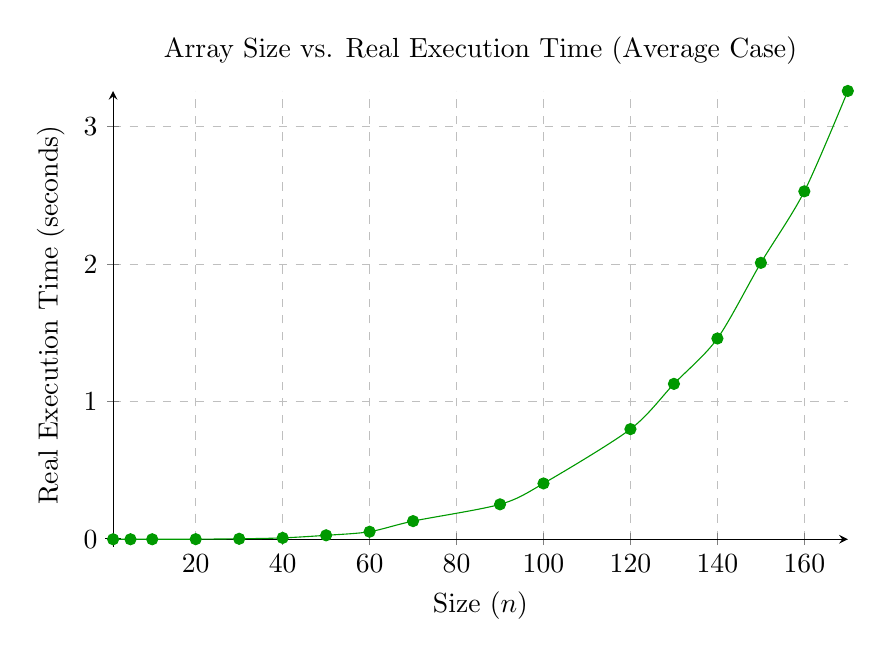
\begin{tikzpicture}
		\begin{axis}[
			% Axis labels and title
			title={Array Size vs. Real Execution Time (Average Case)},
			xlabel={Size (\(n\))},
			ylabel={Real Execution Time (seconds)},
			% Axis limits
			%xmin=0, xmax=100,
			ymin=0, %ymax=200,
			% Axis ticks
			% xtick={0,20,40,60,80,100},
			% ytick={0,20,40,60,80,100,120},
			grid=both,
			axis lines=left,
			axis line style={|-stealth},
			grid style=dashed,
			width=0.9\textwidth,
			height=\axisdefaultheight
			]
			\addplot[
				color=green!60!black,
				mark=*,
				smooth
				]
			% Change the coordinates here with your own data:
			coordinates {
				(1, 0.000000596)
				(5,   0.00000553)
				(10,  0.0000539)
				(20,  0.000734)
				(30,  0.00345)
				(40,  0.00999)
				(50,  0.0288)
				(60,  0.0549)
				(70,  0.132)
				(90,  0.254)
				(100, 0.406)
				(120, 0.801)
				(130, 1.13)
				(140, 1.46)
				(150, 2.01)
				(160, 2.53)
				(170, 3.26)
			};
		\end{axis}
	\end{tikzpicture}
	\end{figure}
	
	\subsubsection{Graph of the theoretical analysis when basic operation is the operation marked as (1)}

 \begin{figure}[H]
	\centering
	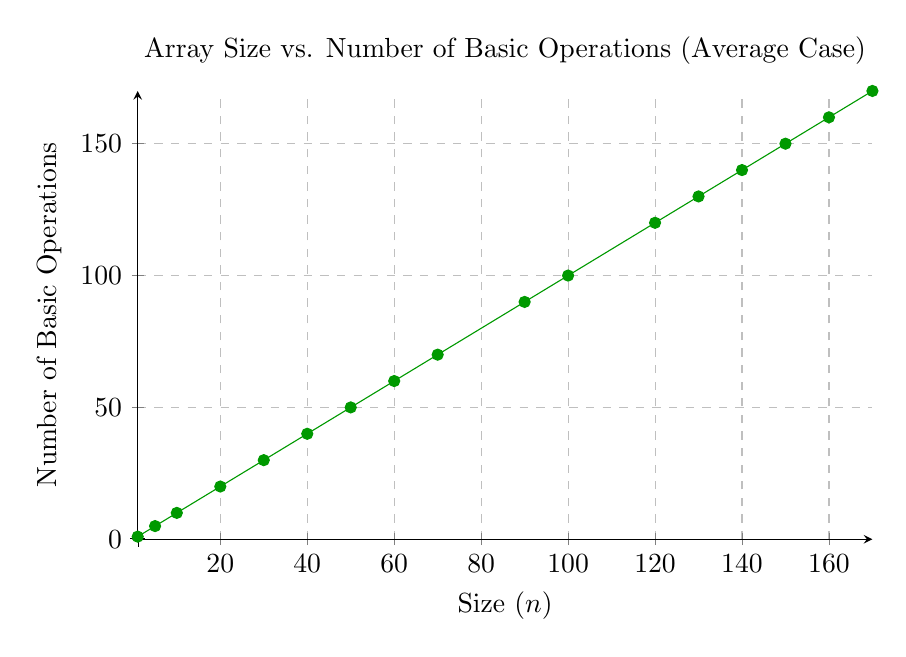
\begin{tikzpicture}
		\begin{axis}[
			% Axis labels and title
			title={Array Size vs. Number of Basic Operations (Average Case)},
			xlabel={Size (\(n\))},
			ylabel={Number of Basic Operations},
			% Axis limits
			%xmin=0, xmax=100,
			ymin=0, %ymax=200,
			% Axis ticks
			% xtick={0,20,40,60,80,100},
			% ytick={0,20,40,60,80,100,120},
			grid=both,
			axis lines=left,
			axis line style={|-stealth},
			grid style=dashed,
			width=0.9\textwidth,
			height=\axisdefaultheight
			]
			\addplot[
				color=green!60!black,
				mark=*,
				smooth
				]
			% Change the coordinates here with your own data:
			coordinates {
				(1,   1)
				(5,   5)
				(10,  10)
				(20, 20)
				(30,  30)
				(40, 40)
				(50,  50)
				(60,  60)
				(70,  70)
				(90,  90)
				(100,100)
				(120, 120)
				(130, 130)
				(140, 140)
				(150, 150)
				(160, 160)
				(170,170)
			};
		\end{axis}
	\end{tikzpicture}
	\end{figure}

	\subsubsection{Graph of the theoretical analysis when basic operation is the operation marked as (2)}

  \begin{figure}[H]
	\centering
	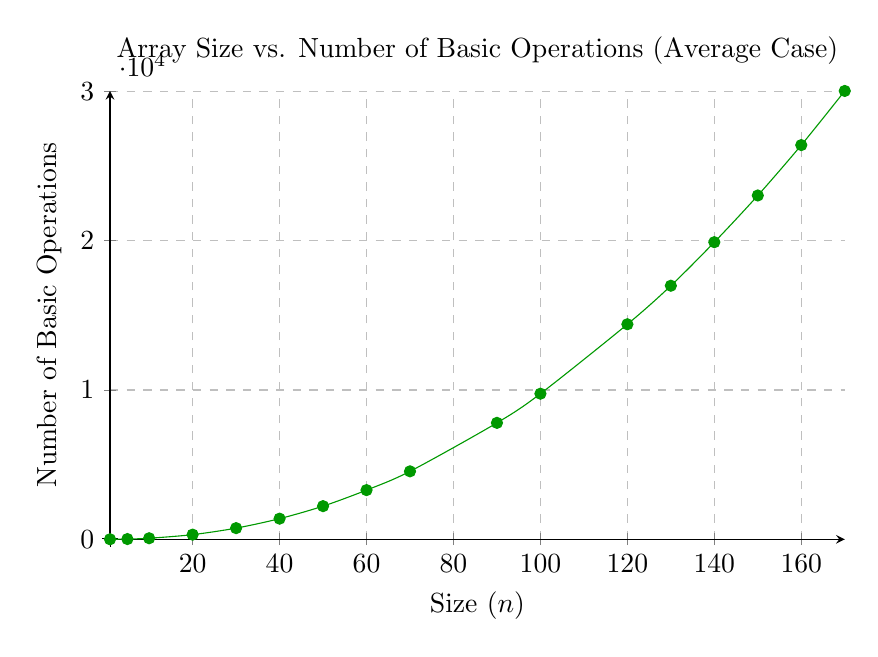
\begin{tikzpicture}
		\begin{axis}[
			% Axis labels and title
			title={Array Size vs. Number of Basic Operations (Average Case)},
			xlabel={Size (\(n\))},
			ylabel={Number of Basic Operations},
			% Axis limits
			%xmin=0, xmax=100,
			ymin=0, %ymax=200,
			% Axis ticks
			% xtick={0,20,40,60,80,100},
			% ytick={0,20,40,60,80,100,120},
			grid=both,
			axis lines=left,
			axis line style={|-stealth},
			grid style=dashed,
			width=0.9\textwidth,
			height=\axisdefaultheight
			]
			\addplot[
				color=green!60!black,
				mark=*,
				smooth
				]
			% Change the coordinates here with your own data:
			coordinates {
				(1,   0.25)
				(5,   14.375)
				(10,  68.75)
				(20, 310)
				(30,  746.25)
				(40, 1380)
				(50,  2218.75)
				(60,  3292.5)
				(70,  4550)
				(90,  7796.25)
				(100,9750)
				(120, 14400)
				(130, 16981.25)
				(140, 19897.5)
				(150, 23025)
				(160, 26400)
				(170,30026.25)
			};
		\end{axis}
	\end{tikzpicture}
	\end{figure}

	\subsubsection{Graph of the theoretical analysis when basic operation is the operation marked as (3)}

  \begin{figure}[H]
	\centering
	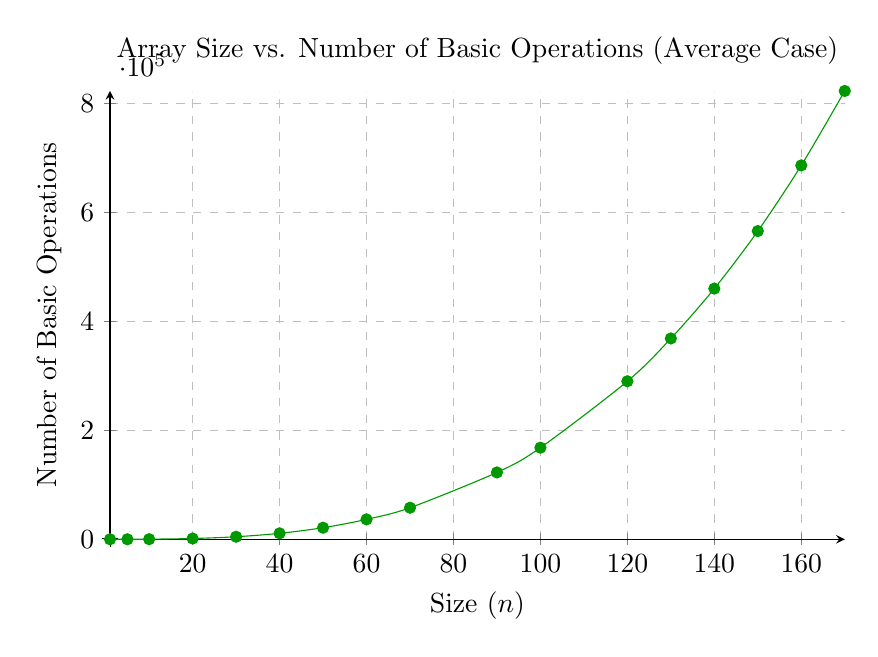
\begin{tikzpicture}
		\begin{axis}[
			% Axis labels and title
			title={Array Size vs. Number of Basic Operations (Average Case)},
			xlabel={Size (\(n\))},
			ylabel={Number of Basic Operations},
			% Axis limits
			%xmin=0, xmax=100,
			ymin=0, %ymax=200,
			% Axis ticks
			% xtick={0,20,40,60,80,100},
			% ytick={0,20,40,60,80,100,120},
			grid=both,
			axis lines=left,
			axis line style={|-stealth},
			grid style=dashed,
			width=0.9\textwidth,
			height=\axisdefaultheight
			]
			\addplot[
				color=green!60!black,
				mark=*,
				smooth
				]
			% Change the coordinates here with your own data:
			coordinates {
				(1,   0.25)
				(5,   28.125)
				(10,  190)
				(20, 1410)
				(30,  4656.25)
				(40, 10935)
				(50,  21231.25)
				(60,  36552.5)
				(70,  57916.25)
				(90,  122688.75)
				(100,168112.5)
				(120, 290035)
				(130, 368582.5)
				(140, 460110)
				(150, 565662.5)
				(160, 686240)
				(170,822842.5)
			};
		\end{axis}
	\end{tikzpicture}
	\end{figure}

	\subsubsection{Graph of the theoretical analysis when basic operation is the operation marked as (4)}

  \begin{figure}[H]
	\centering
	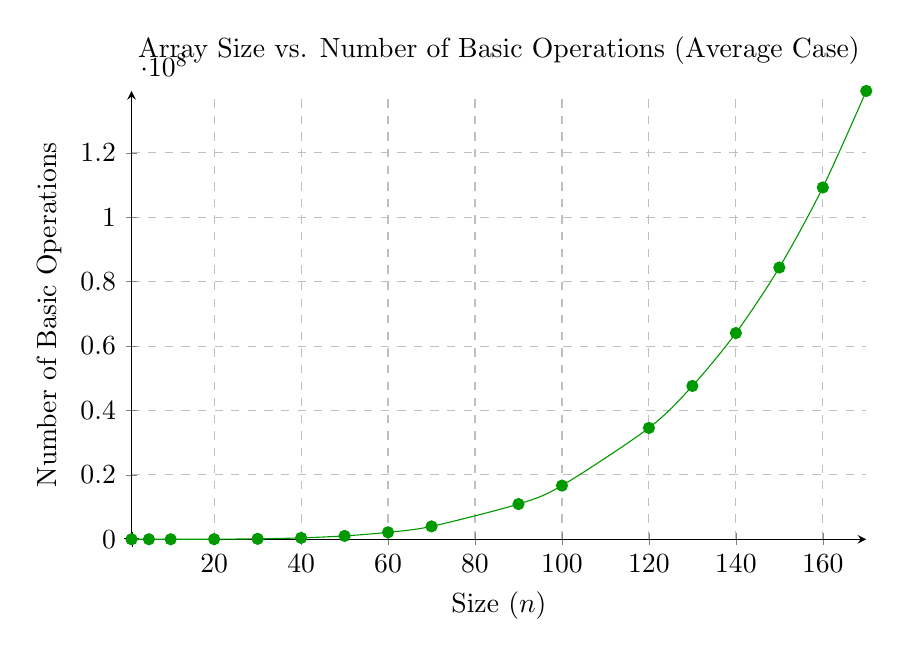
\begin{tikzpicture}
		\begin{axis}[
			% Axis labels and title
			title={Array Size vs. Number of Basic Operations (Average Case)},
			xlabel={Size (\(n\))},
			ylabel={Number of Basic Operations},
			% Axis limits
			%xmin=0, xmax=100,
			ymin=0, %ymax=200,
			% Axis ticks
			% xtick={0,20,40,60,80,100},
			% ytick={0,20,40,60,80,100,120},
			grid=both,
			axis lines=left,
			axis line style={|-stealth},
			grid style=dashed,
			width=0.9\textwidth,
			height=\axisdefaultheight
			]
			\addplot[
				color=green!60!black,
				mark=*,
				smooth
				]
			% Change the coordinates here with your own data:
			coordinates {
				(1,   0.375)
				(5,   114.375)
				(10,  1708.75)
				(20, 26845)
				(30,  135427.5)
				(40, 427465)
				(50,  1042950)
				(60,  2161920)
				(70,  4004341.25)
				(90,  10939635)
				(100,16672487.5)
				(120, 34568685)
				(130, 47611963.75)
				(140, 64038782.5)
				(150, 84389062.5)
				(160, 109242840)
				(170,139220118.75)
			};
		\end{axis}
	\end{tikzpicture}
	\end{figure}



	\subsubsection{Comments}

\end{document}
